\documentclass[12pt]{article}

\usepackage[margin=1in]{geometry}
\usepackage{amsmath,amsthm,amssymb}
\usepackage{float}
\usepackage{graphicx}

\newcommand{\N}{\mathbb{N}}
\newcommand{\Z}{\mathbb{Z}}
\newcommand{\abs}[1]{\left| #1 \right|}
\newcommand{\ceil}[1]{\left\lceil #1 \right\rceil}
\newcommand{\floor}[1]{\left\lfloor #1 \right\rfloor}
\newcommand{\pprime}{\prime \prime}
\newcommand{\BigO}[1]{\mathcal{O}\left( #1 \right)}

\newenvironment{theorem}[2][Theorem]{\begin{trivlist}
\item[\hskip \labelsep {\bfseries #1}\hskip \labelsep {\bfseries #2.}]}{\end{trivlist}}
\newenvironment{lemma}[2][Lemma]{\begin{trivlist}
\item[\hskip \labelsep {\bfseries #1}\hskip \labelsep {\bfseries #2.}]}{\end{trivlist}}
\newenvironment{exercise}[2][Exercise]{\begin{trivlist}
\item[\hskip \labelsep {\bfseries #1}\hskip \labelsep {\bfseries #2.}]}{\end{trivlist}}
\newenvironment{problem}[2][Problem]{\begin{trivlist}
\item[\hskip \labelsep {\bfseries #1}\hskip \labelsep {\bfseries #2.}]}{\end{trivlist}}
\newenvironment{question}[2][Question]{\begin{trivlist}
\item[\hskip \labelsep {\bfseries #1}\hskip \labelsep {\bfseries #2.}]}{\end{trivlist}}
\newenvironment{corollary}[2][Corollary]{\begin{trivlist}
\item[\hskip \labelsep {\bfseries #1}\hskip \labelsep {\bfseries #2.}]}{\end{trivlist}}

\DeclareMathOperator{\sech}{sech}
\DeclareMathOperator{\csch}{csch}

\begin{document}

\title{CS6210: Homework 2}
\author{Christopher Mertin}
\date{September 15, 2016}
\maketitle

\begin{enumerate}
%%%%%% Problem 1 %%%%%%
\item Consider the fixed point iteration $x_{k+1} = g\left( x_{k}\right),\ k=\{0,1,\ldots\}$
and let all the assumptions of the Fixed Point Theorem hold. Use a Taylor's series expansion
to show that the order of convergence depends on how many of the derivatives of $g$ vanish
at $x = x^{*}$. Use your result to state how fast (at least) a fixed point iteration
is expected to converge if $g^{\prime} = \cdots = g^{(r)}\left( x^{*}\right) = 0$,
where the integer $r \geq 1$ is given.

{\bf Solution:}

The definition of the Taylor Series Expansion for a function $g(x)$ around $x = x^{*}$ is defined as:

\begin{align*}
g(x) &= \sum_{n=0}^{\infty} \frac{g^{(n)}\left( x^{*}\right)}{n!} \left( x - x^{*}\right)^{n}\\
g\left( x_{k}\right) &= \sum_{n=0}^{\infty} \frac{g^{(n)}\left( x^{*}\right)}{n!} \left( x_{k} - x^{*}\right)^{n}\\
x_{k+1} - x^{*} &= \xi_{k+1} = \sum_{n=0}^{\infty} \frac{g^{(n)}\left( x^{*}\right)}{n!}\xi_{k}^{n}
\intertext{If $g^{\prime}\left( x^{*}\right) = 0$, then}
\xi_{k+1} &= \sum_{n=2}^{\infty} \frac{g^{(n)}\left( x^{*}\right)}{n!} \xi_{k}^n = \xi_{k}^{2}\sum_{n=2}^{\infty}\frac{g^{(n)}\left( x^{*}\right)}{n!}\xi_{k}^{n-2}
\end{align*}

Which shows that $g(x)$ is {\em minimally} quadratically convergent. Consequently, if
$g^{(i)}\left( x^{*}\right) = 0$ for $i \in \{1,2,\ldots,r\}$, then the function has a
divergence of {\em at least} $\BigO{r}$.

%%%%%% Problem 2 %%%%%%
\item Consider the function $g(x) = x^{2} + \frac{3}{16}$

\begin{enumerate}
  \item This function has two fixed points. What are they?

  {\bf Solution:}

  In order to find the {\em fixed points} of the above function, we need to find
  the zeros

  \begin{align*}
    x^{2} + \frac{3}{16} &= x\\
    x^{2} - x + \frac{3}{16} &= 0\\
    \Rightarrow x_{1} &= \frac{1}{4}\\
    \Rightarrow x_{2} &= \frac{3}{4}
  \end{align*}
  \item Consider the fixed point iteration $x_{k+1} = g\left( x_{k}\right)$ for this $g$.
  For which of the points you have found in $(a)$ can you be sure that the iterations
  will converge to that fixed point? Briefly justify your answer. You may assume that
  the initial guess is sufficiently close to the fixed point.

{\bf Solution:}

  Since the inital guess is said to be {\em sufficiently close to the fixed point},
  we can assume that the given range is the following.

  \begin{align*}
    \frac{1}{4} &\leq x \leq \frac{3}{4}
  \end{align*}
  We need to check to make sure the function $f(x)$ is constrained in this domain, such that it won't go ``over'' or ``under'' when getting the next $x_{k+1}$ point. To do so
  \begin{align*}
    \frac{1}{16} &\leq x^{2} \leq \frac{9}{16}\\
    \frac{1}{16} + \frac{3}{16} &\leq x^{2} + \frac{3}{16} \leq \frac{9}{16} + \frac{3}{16}\\
    \frac{1}{4} &\leq f(x) \leq \frac{3}{4}
    \end{align*}

    So $f(x)$ is contained in the interval $\frac{1}{4} \leq f(x) \leq \frac{3}{4}$ for
    choosing an initial $x$ in the same interval. Therefore, we can now check to see if it will
    converge to each of the fixed points by checking the {\em slope} of the function

    \begin{align*}
      g^{\prime}(x) &= 2x\\
      g^{\prime}\left(\frac{1}{4}\right) &= \frac{1}{2}\\
      g^{\prime}\left(\frac{3}{4}\right) &= \frac{3}{2}
    \end{align*}

    Since $g^{\prime}\left(\frac{1}{4}\right) < 1$, it is a decreasing slope and the function will converge
    for $x_{1} = \frac{1}{4}$. Like wise, $g^{\prime}\left(\frac{3}{4}\right) > 1$ means that it will converge
    to $x_{2} = \frac{3}{4}$, assuming that the initial value is {\em sufficiently close}.
  \item For the point or points you found in $(b)$, roughly how many iterations will be
  required to reduce the convergence error by a factor of 10?

  {\bf Solution:}

  Page 49 of the text gives the equation to reduce the convergence error by a factor of 10.
  The number of iterations is defined as $k = \ceil{1/rate}$, for which $rate = -\log_{10}\abs{g^{\prime}\left( x^{*}\right)}$.
  Using this equation, we can get the convergence rate to be

  \begin{align*}
    g^{\prime}\left( \frac{1}{4}\right) &= \frac{1}{2}\\
    \Rightarrow rate &= -\log_{10}\abs{2^{-1}} = \frac{3}{10}\\
    \intertext{So it takes $k = \ceil{1/rate}$ iterations to reduce the error by more than an order of magnitude, resulting in}
    k &= \ceil{\left( \frac{3}{10}\right)^{-1}} = 4
  \end{align*}
\end{enumerate}

%%%%%% Problem 3 %%%%%%
\item It is known that the order of convergence of the secant method is $p = \frac{1 + \sqrt{5}}{2} \approx 1.618\ldots$
and that of Newton's method is $p = 2$. Suppose that evaluating $f^{\prime}$ costs approximately
$\alpha$ times the cost of approximating $f$. Determine approximately for what values of $\alpha$
Newton's method is more efficient (in terms of number of function evaluations) than the secant method.
You may neglect the asymptotic error constants in your calculations. Assume that both methods
are starting with initial guesses of a similar quality.

{\bf Solution:}

%%%%%% Problem 4 %%%%%%
\item The function

\[
f(x) = (x-1)^{2}e^{x}
\]

has a double root at $x = 1$.

\begin{enumerate}
\item Derive Newton's iteration for this function. Show that the iteration is well-defined
so long as $x_{k} \neq -1$ and that the convergence rate is expected to be similar to that
of the bisection method (and certainly not quadratic).

{\bf Solution:}

In order to build the methods, we need the following

\begin{align*}
f(x) &= (x-1)^{2}e^{x}\\
f^{\prime}(x) &= (x-1)^{2}e^{x} + 2(x-1)e^{x}\\
f^{\pprime}(x) &= (x-1)^{2}e^{x} + 2(x-1)e^{x} + 2(x-1)^{2}e^{x} + 2e^{x}
\end{align*}

with Newton's method being defined as:

\begin{align*}
x_{k+1} &= x_{k} - \frac{f\left(x_{k}\right)}{f^{\prime}\left(x_{k}\right)}\\
        &= x_{k} - \frac{\left(x_{k}-1\right)^{2}e^{x_{k}}}{2\left(x_{k}-1\right)e^{x_{k}} + \left( x_{k} - 1\right)^{2}e^{x_{k}}}\\
        &= x_{k} - \frac{x_{k}-1}{x_{k} + 1}
\end{align*}

Which shows that it is well defined {\em except} for $x_{k} = -1$. We can subtract the approximation
of the root for $x = 1$ of $f(x)$ from both sides, which gives

\begin{align*}
x_{k+1} - x^{*} &= x_{k} - \frac{x_{k} - 1}{x_{k} + 1} - x^{*}\\
\xi_{k+1} &= \xi_{k} - \frac{x_{k}-1}{x_{k}+1} \approx \xi_{k} - \frac{x_{k} - x^{*}}{x_{k}+1}\\
          &= \xi_{k} - \frac{\xi_{k}}{x_{k}+1} = \xi_{k} \left( 1 - \frac{1}{x_{k}+1}\right)\\
          &= \xi_{k}\left( \frac{x_{k}}{x_{k}+1}\right)
\end{align*}

With $\frac{x_{k}}{x_{k}+1} < 1$, it is not quadratically convergent.

\item Implement Newton's method and observe its performance starting from $x_{0} = 2$.

{\bf Solution:}

\begin{figure}[H]
\centering
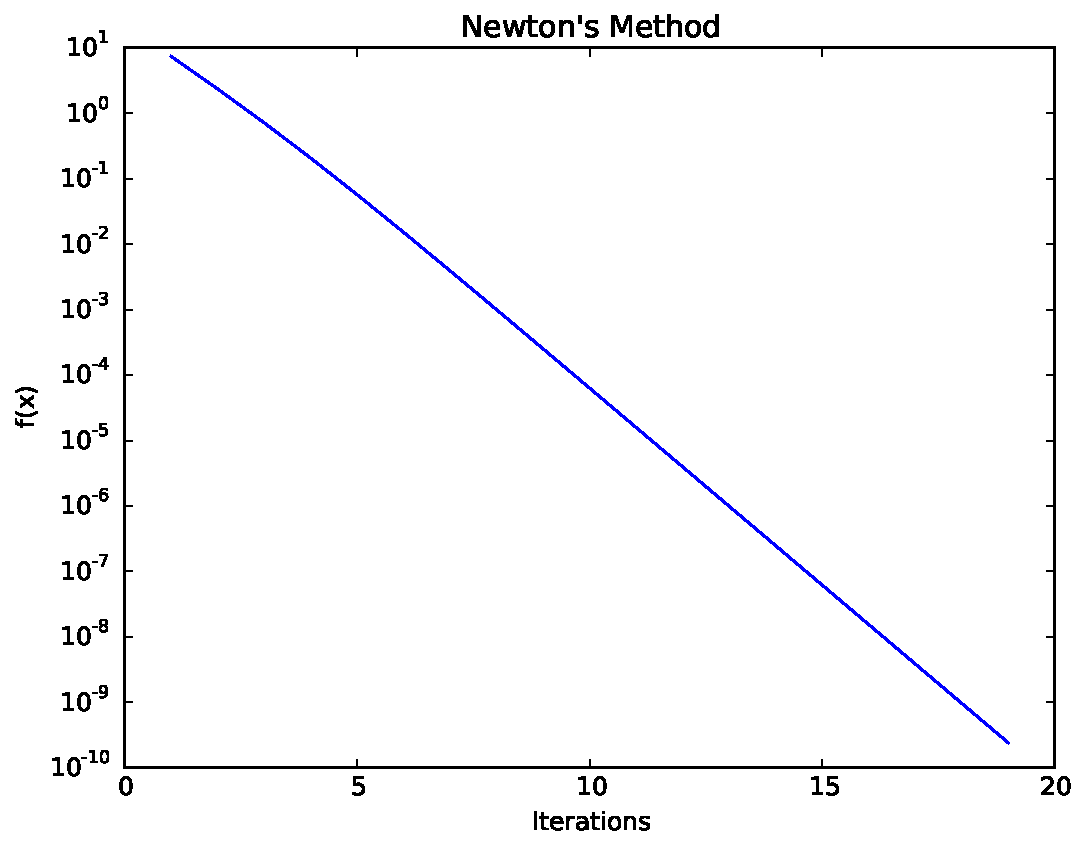
\includegraphics[width = .65\textwidth]{hw2_prob4.pdf}
\caption{{\tt prob4.py}}
\end{figure}

\item How easy would it be to apply the bisection method? Explain.

{\bf Solution:}

To use the Bisection Method, we need two points $x_{0}$ and $x_{1}$ in the domain.
It is also required that $f\left(x_{0}\right)$ has a different sign than $f\left(x_{1}\right)$,
which since $f(x)$ is positive over the entire domain, cannot hold true. Therefore, the Bisection Method
cannot be used.

\end{enumerate}

%%%%%% Problem 5 %%%%%%
\item Given $a > 0$, we wish to compute $x = \ln (a)$ using addition, subtraction, multiplication,
division, and the exponential function $e^{x}$.
\begin{enumerate}
\item Suggest an iterative formula based on Newton's method, and write it in a way suitable
for numerical computation.

{\bf Solution:}

In order to find an iterative formula, we need an $f(x)$ such that $f(x) = 0$ at some point,
and has a derivative in the domain of interest. We can do that by taking the above equation and solving for 0, thus giving the $f(x)$

\begin{align*}
x &= \ln(a)\\
e^{x} &= e^{\ln (a)}\\
\therefore f(x) &= e^{x} - a\\
f^{\prime}(x) &= e^{x}
\end{align*}

As we have a derivative, we can define the Newton's Method for this equation as being

\begin{align*}
x_{k+1} &= x_{k} - \frac{f(x_{k})}{f^{\prime}(x_{k})}\\
        &= x_{k} - \frac{e^{x_{k}} - a}{e^{x_{k}}}\\
        &= x_{k} - \frac{a}{e^{x_{k}}} - 1
\end{align*}

\item Show that your formula converges quadratically.

{\bf Solution:}

We can define $g(x) = \frac{a}{e^{x}} - 1$, and then take the Taylor Series of it, giving

\begin{align*}
  g(x) &= \sum_{n=0}^{\infty}\frac{g^{(n)}\left( x^{*}\right)}{n!}\left(x - x^{*}\right)^{n}\\
  \intertext{For $n=0$ we get $g\left(x^{*}\right) = 0$ and for $n=1$ we get $g^{\prime}\left(x^{*}\right) = -1$, this changes our series to}
  g\left(x_{k}\right) &= 0 - \xi_{k} + \sum_{n=2}^{\infty} \frac{g^{(n)}\left(x^{*}\right)}{n!}\xi_{k}^{n}
  \intertext{where we can replace this into the iterative equation from above, giving}
  x_{k+1} &= x_{k} - \xi_{k} + \sum_{n=2}^{\infty} \frac{g^{(n)}\left(x^{*}\right)}{n!}\xi_{k}^{n}\\
          &= x_{k} - \xi_{k} + \xi_{k}^{2}\sum_{n=2}^{\infty} \frac{g^{(n)}\left(x^{*}\right)}{n!}\xi_{k}^{n-2}\\
  \intertext{Finally, after subtracting $x^{*}$ from both sides, gives}
  \xi_{k+1} = x_{k+1} - x^{*} &= \xi_{k} - \xi_{k} + \xi_{k}^{2}\sum_{n=2}^{\infty} \frac{g^{(n)}\left(x^{*}\right)}{n!}\xi_{k}^{n-2}\\
                              &= \xi_{k}^{2}\sum_{n=2}^{\infty} \frac{g^{(n)}\left(x^{*}\right)}{n!}\xi_{k}^{n-2}
\end{align*}

So it is quadratically convergent.

\item Write down an iterative formula based on the secant method.

{\bf Solution:}

\begin{align*}
x_{k+1} &= x_{k} - \frac{f\left(x_{k}\right) \left(x_{k} - x_{k-1}\right)}{f\left(x_{k}\right) - f\left(x_{k-1}\right)}\\
        &= x_{k} - \frac{\left(e^{x_{k}} - a\right)\left(x_{k} - x_{k-1}\right)}{e^{x_{k}} - a - \left(e^{x_{k-1}} - a\right)}\\
        &= x_{k} - \frac{\left(e^{x_{k}} - a\right)\left(x_{k} - x_{k-1}\right)}{e^{x_{k}} - e^{x_{k-1}}}
\end{align*}

\item State which of the secant and Newton's methods is expected to perform better in
this case in terms of overall number of exponential function evaluations. Assume a fair
comparison, {\em i.e.} same floating point system, ``same quality'' initial guesses, and idential
convergence criterion.

{\bf Solution:}

Newton's method only has two evaluations of the exponential function $\left(f(x)\ \text{and}\ \frac{\text{d}}{\text{d}x}f(x) \right)$
while the Secant Method has three. Thus, Newton's Method should perform better.


\end{enumerate}

%%%%%% Problem 6 %%%%%%
\item For $x>0$ consider the equation

\[
x + \ln(x) = 0
\]

It is a reformulation of the equation of Example 3.4

\begin{enumerate}
  \item Show analytically that there is exactly one root, $0 < x^{*} < \infty$

  {\bf Solution:}

  $\ln(x)$ is a continuous function for $x > 0$, and we can choose two points such that
  $x_{0} = \frac{1}{2}$ and $x_{1} = 1$.

  \begin{align*}
    f\left( x_{0}\right) &\approx \frac{1}{2} - 0.69 < 0\\
    f\left( x_{1}\right) &= 1 + 0 > 0
  \end{align*}

  By the {\em Intermediate Value Theorem}, there must exist some $f(c)$ such that
  $f(c) = 0$ due to the sign change of the function.

  \item Plot a graph of the function on the interval $[0.1, 1]$

  {\bf Solution:}

  \begin{figure}
    \centering
    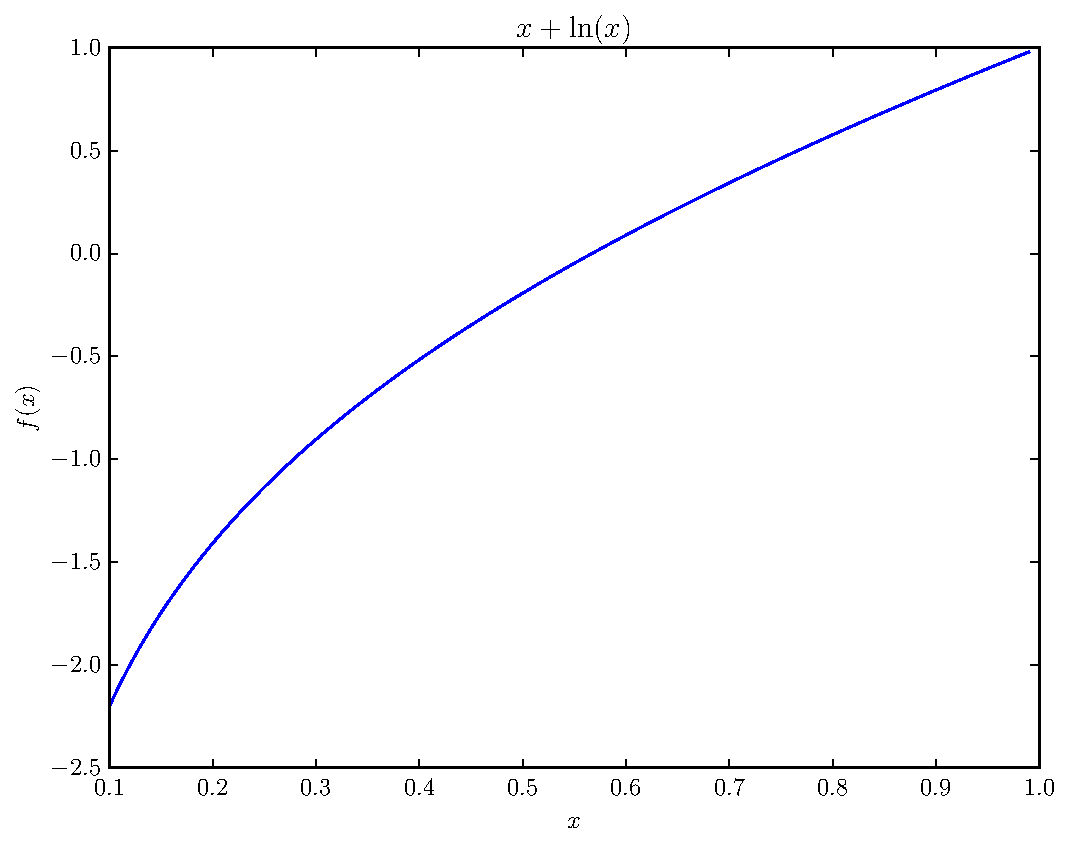
\includegraphics[width=.65\textwidth]{hw2_prob6a.pdf}
  \end{figure}

  \item As you can see from the graph, the root is between $0.5$ and $0.6$. Write
  {\sc Matlab} routines for finding the root, using the following:
  \begin{enumerate}
    \item The bisection method, with the initial interval $[0.5,0.6]$. Explain
    why this choice of the intial interval is valid.

    {\bf Solution:}

    This interval is valid because the sign changes in the domain $[0.5, 0.6]$ so
    the Bisection method can be used. For the plot, please see the last question.

    \item A linearly convergent fixed point interation, with $x_{0} = 0.5$. Show that
    the conditions of the Fixed Point Theorem (for the function $g$ you have selected)
    are satisfied.

    {\bf Solution:}

    In determining $g(x)$, we wanted a function such that $g\left(x^{*}\right) = x^{*}$,
    which was determined in the following way

    \begin{align*}
      x + \ln(x) &= 0\\
      -x &= \ln(x)\\
      x &= e^{-x}
    \end{align*}

    So $g\left( x^{*}\right) = e^{x^{*}}$ since $e^{x^{*}} = x^{*}$ for the given equation.
    This satisfies the conditions of the Fixed Point Method, and can be used to
    converge to the root.
    
    For the plot, please see the last question.

    \item Newton's method, with $x_{0} = 0.5$.

    {\bf Solution:}

    For the plot, please see the last question.

    \item The secant method, with $x_{0} = 0.5$ and $x_{1} = 0.6$.

    {\bf Solution:}

    \begin{figure}[H]
      \centering
      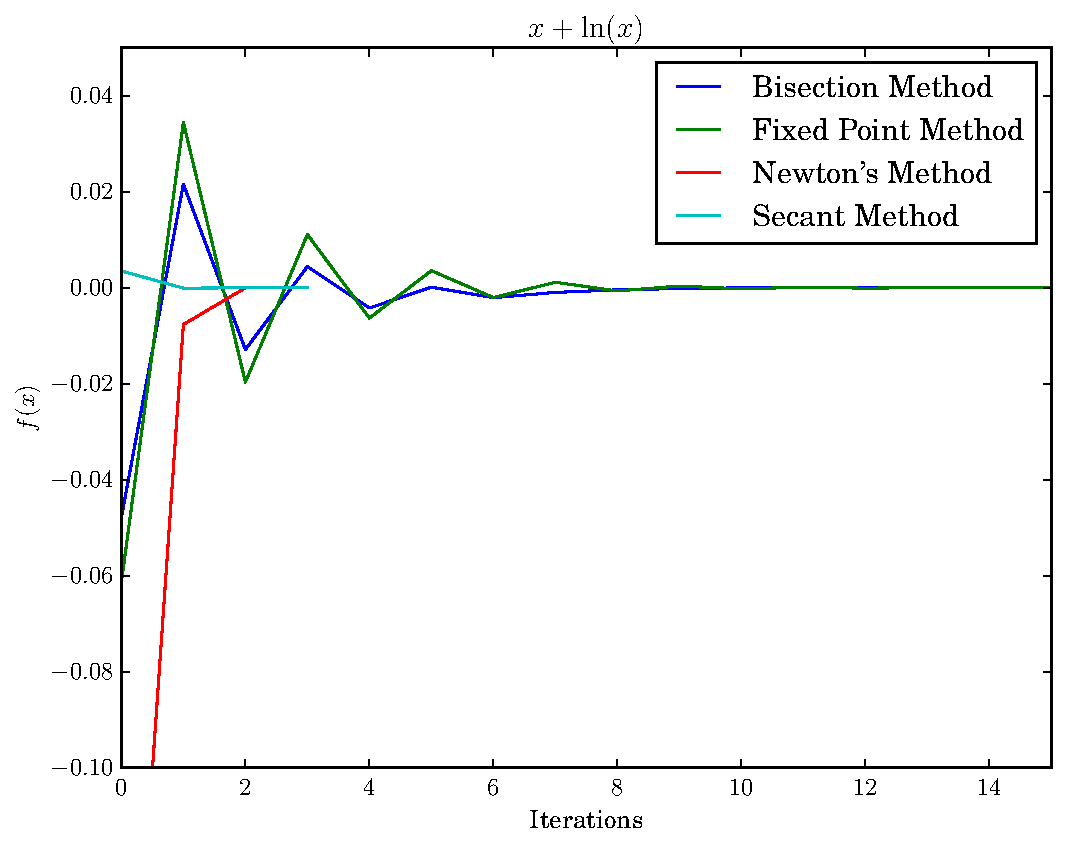
\includegraphics[width=.65\textwidth]{hw2_prob6b.pdf}
      \caption{{\tt prob6.py}}
    \end{figure}


  \end{enumerate}
  For each of the methods:
  \begin{itemize}
    \item Use $\abs{ x_{k} - x_{k-1}} < 10^{-10}$ as convergence criterion
    \item Print out eh iterates and show the progress in the number of correct decimal
    digits throughout the iteration.
    \item Explain the convergence behavior and how it matches theoretical expectations
  \end{itemize}
\end{enumerate}
\end{enumerate}

%\begin{proof}
%Blah, blah, blah.  Here is an example of the \texttt{align} environment:
%Note 1: The * tells LaTeX not to number the lines.  If you remove the *, be sure to remove it below, too.
%Note 2: Inside the align environment, you do not want to use $-signs.  The reason for this is that this is already a math environment. This is why we have to include \text{} around any text inside the align environment.
%\begin{align*}
%\sum_{i=1}^{k+1}i & = \left(\sum_{i=1}^{k}i\right) +(k+1)\\
%& = \frac{k(k+1)}{2}+k+1 & (\text{by inductive hypothesis})\\
%& = \frac{k(k+1)+2(k+1)}{2}\\
%& = \frac{(k+1)(k+2)}{2}\\
%& = \frac{(k+1)((k+1)+1)}{2}.
%\end{align*}
%\end{proof}

\end{document}
